
\documentclass{ximera}

\input{../../preamble.tex}

\author{Ivo Terek}
\license{Creative Commons Attribution-ShareAlike 4.0 International License}

%\outcome{Calculating the rate of change.}
%\outcome{Discuss the meaning of antiderivatives of a position function.}

\begin{document}
\begin{exercise}

<<<<<<< HEAD
If the graph of $y=f(x) = e^{-x}$ is given in black below, which of the following graphs could be the graph of $y = f(x)+3$?
=======
If the graph of $y=f(x)$ is given in black below, which of the following graphs could be the graph of $y = f(x)+3$?
>>>>>>> origin/cleaning

  \begin{image}
 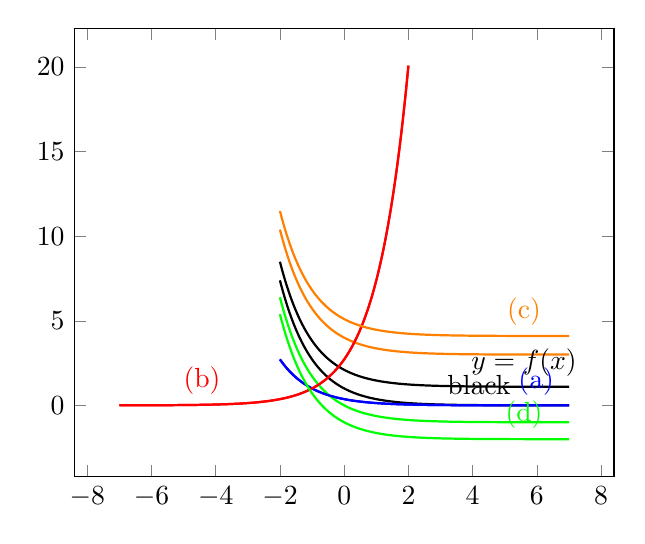
\begin{tikzpicture}
   \begin{axis}
<<<<<<< HEAD
     \addplot [samples=200, thick, domain=-2:7] {exp(-x)} node[pos=0.8,above]{\text{black}};
     \addplot [samples=200, thick,domain=-2:7, color=blue] {exp(-x-1)};
     \addplot [samples=200, thick,domain=-7:2, color=red]{exp(x+1)};
     \addplot [samples=200, thick,domain=-2:7, color=orange]{exp(-x)+3};
     \addplot [samples=200, thick,domain=-2:7, color=green]{exp(-x)-1};
=======
     \addplot [samples=200, thick, domain=-2:7] {exp(-x)+1.1}  node[pos=0.9,above]{\text{$y=f(x)$}};
     \addplot [samples=200, thick,domain=-2:7, color=blue] {exp(-x-1)} node[pos=0.9,above]{\text{(a)}};
     \addplot [samples=200, thick,domain=-7:2, color=red]{exp(x+1)}  node[pos=0.1,above]{\text{(b)}};
     \addplot [samples=200, thick,domain=-2:7, color=orange]{exp(-x)+4.1}  node[pos=0.9,above]{\text{(c)}};
     \addplot [samples=200, thick,domain=-2:7, color=green]{exp(-x)-2} node[pos=0.9,above]{\text{(d)}};
>>>>>>> origin/cleaning
   \end{axis}
 \end{tikzpicture}
 \end{image}

\begin{multipleChoice}
  \choice{Blue graph}
  \choice{Red graph}
  \choice[correct]{Orange graph}
  \choice{Green graph}
\end{multipleChoice}

\end{exercise}
\end{document}